% I commenti sono fatti in modo intenzionale!
% subsection{FrontEnd}
% subsubsection{Controllers}
\label{seqFrontEnd}
Vengono di seguito riportate alcune sequenze di operazioni svolte dai \gloxy{controller} che si è ritenuto utile descrivere più in dettaglio.
\subsubsubsection{RegistrationController - Registrazione di un nuovo utente}
\begin{center}
\begin{figure}[h]
\centering
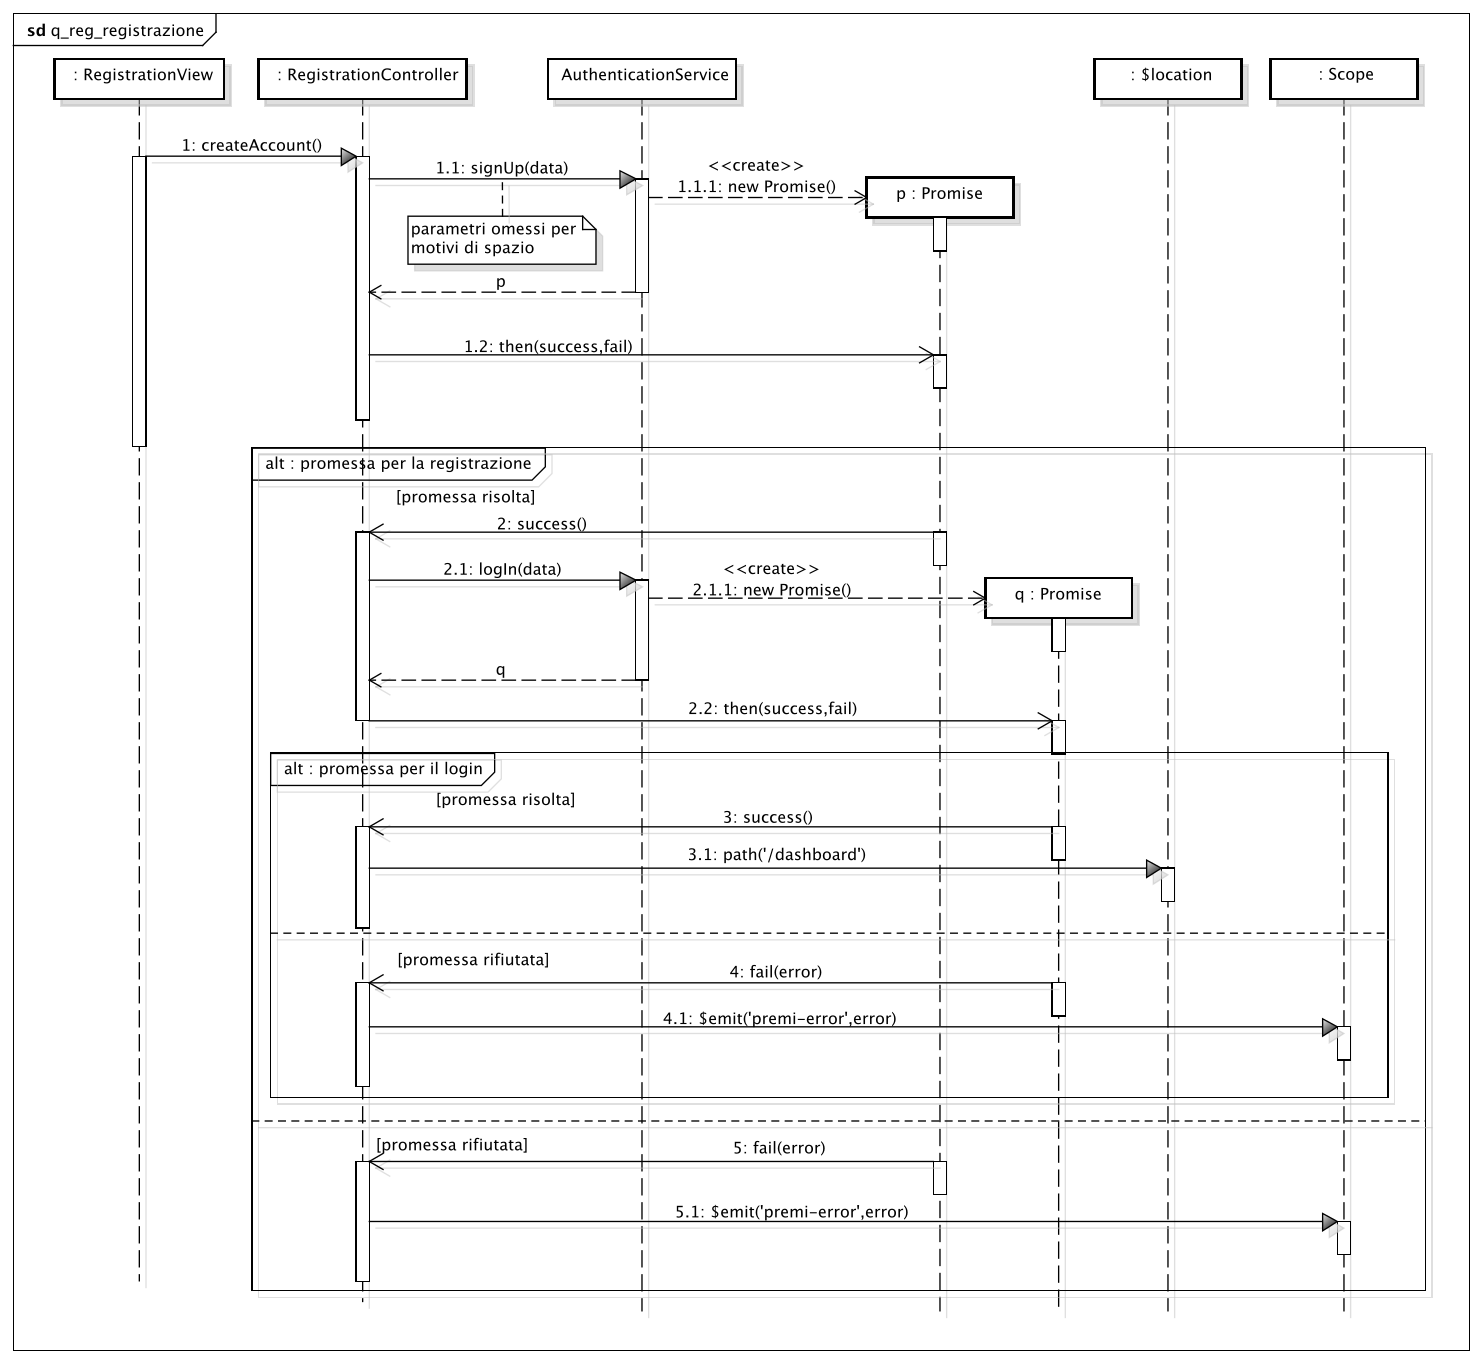
\includegraphics[scale=0.25,keepaspectratio]{diagrammi/sequenza/FrontEnd/controllers/q_reg_registrazione.pdf}
\caption{Diagramma di Sequenza - Registrazione di un nuovo utente}
\end{figure}
\end{center}
\FloatBarrier
Quando l'utente preme il pulsante per la registrazione viene invocato il metodo \texttt{createAccount()}, il quale si preoccupa di andare a leggere i dati inseriti nello \texttt{\$scope} dall'utente e di usarli per invocare il metodo \texttt{signUp} di \texttt{AuthenticationService}.\\
Il service ritorna un oggetto \texttt{Promise} al quale il \gloxy{controller} fornisce due funzioni anonime da invocare nel caso la promessa sia risolta o rifiutata.	\\
Se la promessa viene rifiutata, il \gloxy{controller} solleva l'evento \texttt{premi-error} per segnalare all'utente che non è stato possibile effettuare la registrazione. \\
Se invece la promessa viene soddisfatta, il \gloxy{controller} richiede a \texttt{AuthenticationService} l'autenticazione con gli stessi dati che l'utente ha inserito per registrarsi.\\
Anche in questo caso viene ritornata una promessa e, anche in questo caso, il \gloxy{controller} fornisce all'oggetto \texttt{Promise} due funzioni anonime.\\
Se la promessa viene risolta, il \gloxy{controller} esegue il re-indirizzamento alla dashboard altrimenti, viene sollevato l'evento \texttt{premi-error} per segnalare all'utente l'errore che si è verificato.
\subsubsubsection{DashboardController - Apertura di un progetto}\label{dcap}
\begin{center}
\begin{figure}[h]
\centering
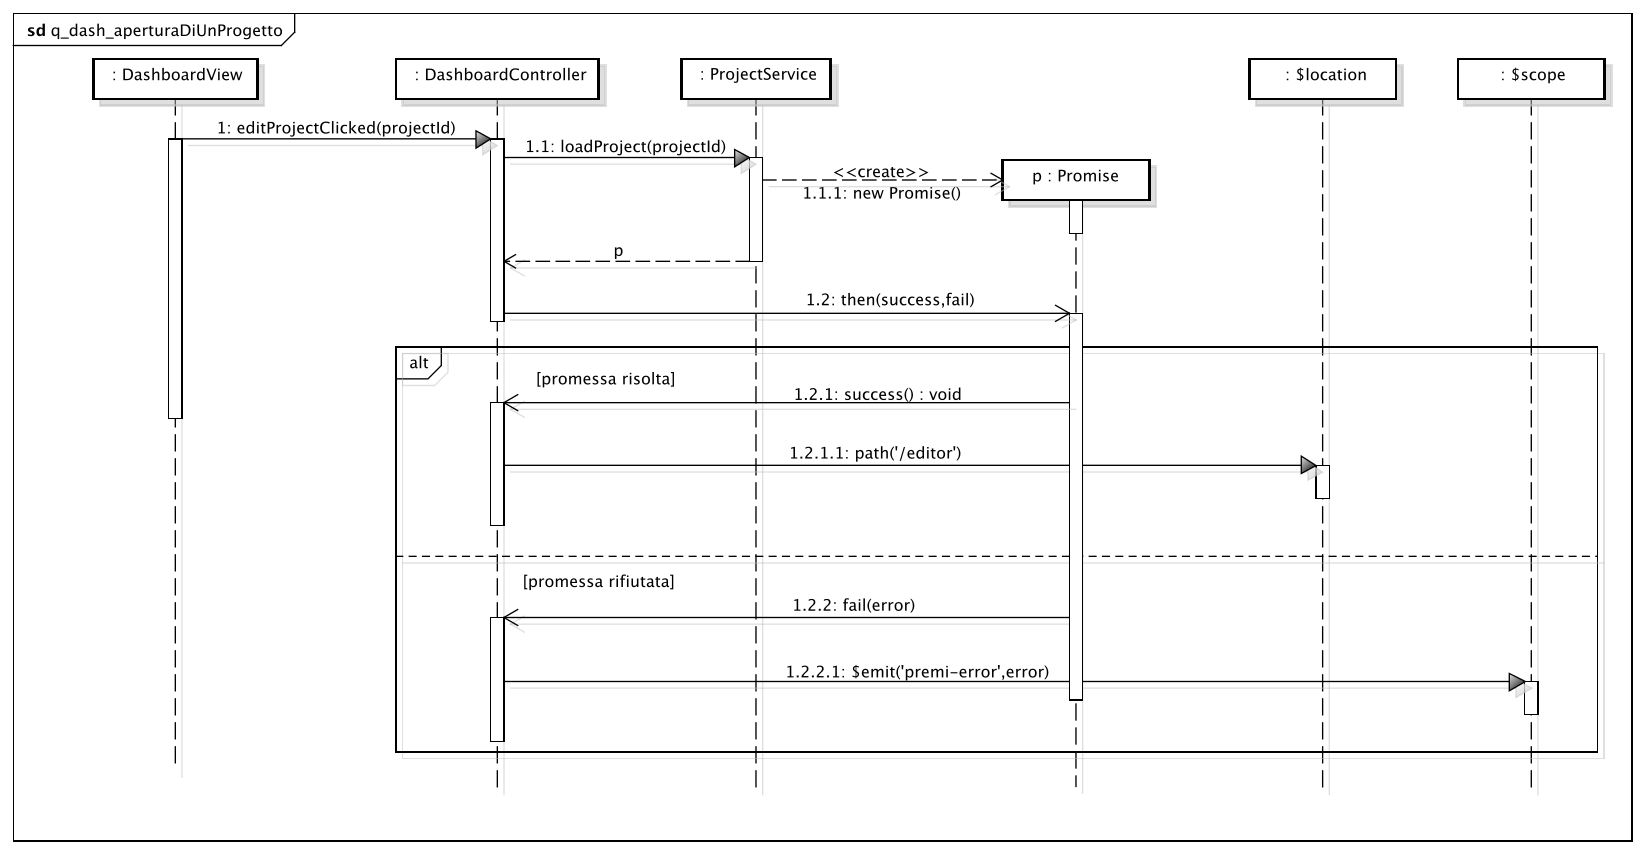
\includegraphics[scale=0.25,keepaspectratio]{diagrammi/sequenza/FrontEnd/controllers/q_dash_aperturaDiUnProgetto.pdf}
\caption{Diagramma di Sequenza - Apertura di un progetto}
\end{figure}
\end{center}
\FloatBarrier
Quando l'utente preme il pulsante per la modifica di un \gloxy{progetto} viene invocato, come gestore dell'evento, il metodo \texttt{editProjectClicked(projectId)}. Questo si preoccupa di richiedere a \texttt{ProjectService} l'apertura del \gloxy{progetto} identificato  da \texttt{projectId}.\\
La funzione del service ritorna un oggetto di tipo \texttt{Promise}, al quale il \gloxy{controller} fornisce due funzioni anonime per gestire la risoluzione o il rifiuto della promessa.\\
Se la promessa viene soddisfatta, il \gloxy{controller} effettua il re-indirizzamento alla pagina per l'editing del \gloxy{progetto}, altrimenti, se la promessa viene rifiutata, il \gloxy{controller} segnala un'errore sollevando l'evento \texttt{premi-error}.
Il re-indirizzamento porta alla costruzione di un \texttt{MindmapEditorController}, la sequenza di operazioni per la costruzione di tale \gloxy{controller} viene descritta nella sezione \ref{edma_l}.
\subsubsubsection{MindmapEditorController - Costruzione del controller}\label{edma_l}
\begin{center}
\begin{figure}[h]
\centering
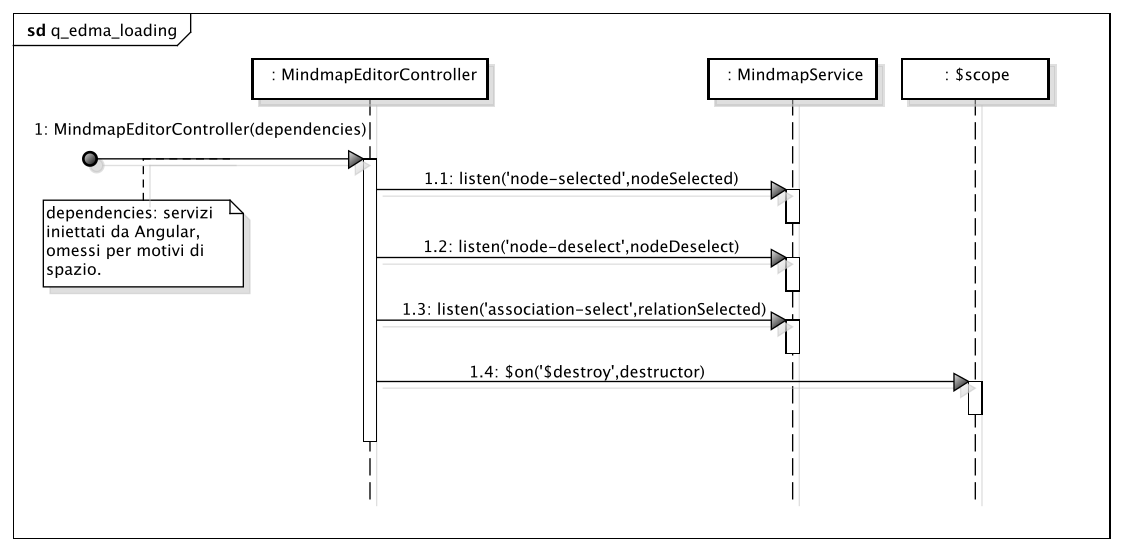
\includegraphics[scale=0.25,keepaspectratio]{diagrammi/sequenza/FrontEnd/controllers/q_edma_loading.pdf}
\caption{Diagramma di Sequenza - Costruzione del controller}
\end{figure}
\end{center}
\FloatBarrier
Quando l'utente apre un \gloxy{progetto} e desidera visualizzarne la \gloxy{mappa mentale} per modificarla deve essere istanziato il \gloxy{controller} legato a quella \gloxy{view}. In particolare viene eseguita questa sequenza di azioni:
\begin{enumerate}
\item Vengono registrate le varie funzioni di \gloxy{callback} per i seguenti eventi offerti da \texttt{MindmapService}:
\begin{itemize}
\item \texttt{node-select};
\item \texttt{node-deselect};
\item \texttt{association-select}.
\end{itemize}
\item Viene registrato il distruttore del \gloxy{controller} sull'evento \texttt{\$destroy} dello \texttt{\$scope}.
\end{enumerate}
Non è necessario recuperare e inizializzare i dati della \gloxy{mappa mentale} in quanto il caricamento dei dati viene effettuato da \texttt{ProjcetService.loadProject} e l'inizializzazione della mappa mentale è delegata alla directive \texttt{premiMindmap}.
%---
\subsubsubsection{MindmapEditorController - Selezione di un nodo}\label{emc}
\begin{center}
\begin{figure}[h]
\centering
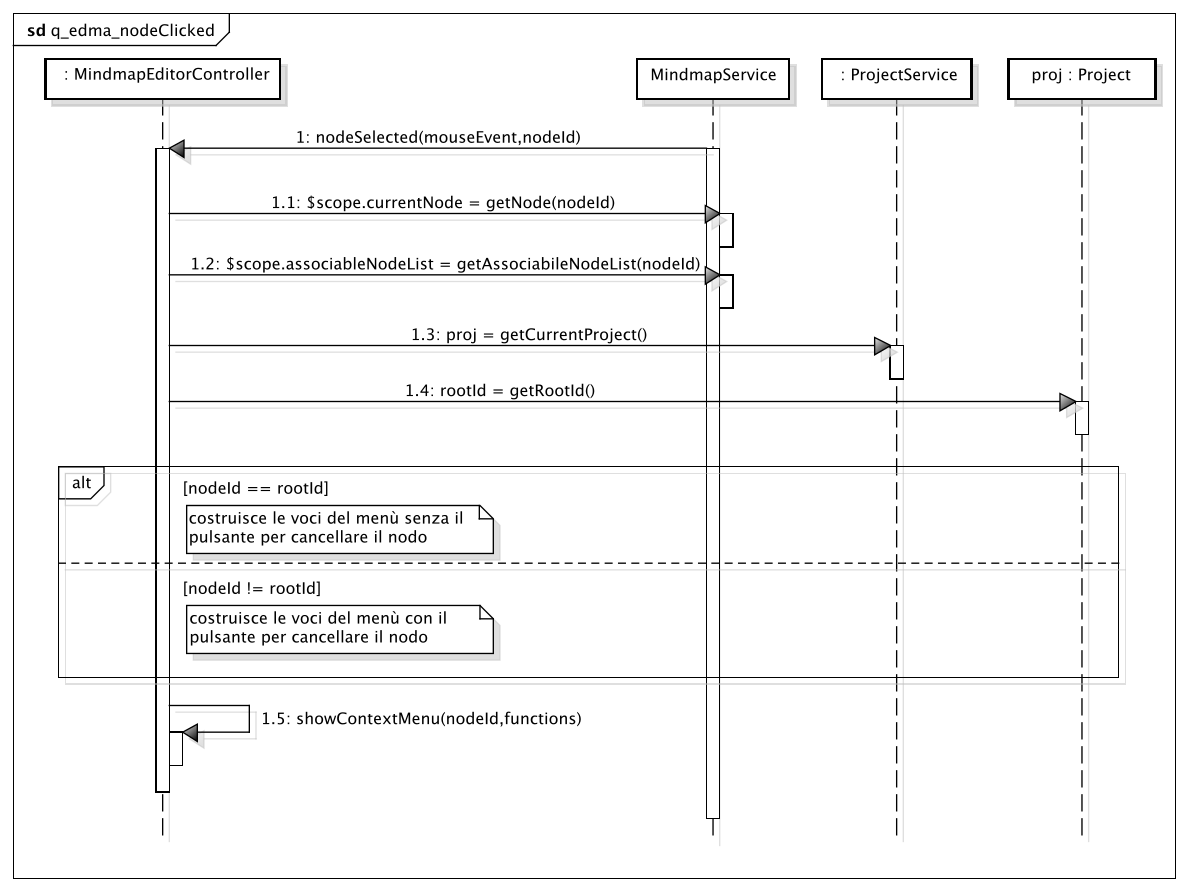
\includegraphics[scale=0.33,keepaspectratio]{diagrammi/sequenza/FrontEnd/controllers/q_edma_nodeClicked.pdf}
\caption{Diagramma di Sequenza - Selezione di un nodo}
\end{figure}
\end{center}
\FloatBarrier
Quando l'utente seleziona un nodo della \gloxy{mappa mentale} il service \texttt{MindmapService} invoca la funzione di \textit{\gloxy{callback}} del \gloxy{controller} in modo che l'evento possa essere gestito correttamente.\\
L'esecuzione delle funzione \texttt{nodeSelected(mouseEvent,nodeId)} deve:
\begin{enumerate}
\item Aggiornare la variabile \texttt{\$scope.currentNode} con il nodo identificato da \texttt{nodeId};
\item Aggiornare la variabile \texttt{\$scope.associableNodeList} con la lista dei nodi che possono essere associati al nodo corrente;
\item Recuperare le informazioni riguardanti il nodo radice del \gloxy{progetto};
\item Caricare le voci del menù e, nel caso il nodo selezionato sia la radice, disabilitare l'eliminazione del nodo;
\item Visualizzare il menù di modifica del nodo invocando la funzione \texttt{showContextMenu}.
\end{enumerate}
\subsubsubsection{PresentationController - Creazione di una presentazione}\label{cdup}
\begin{center}
\begin{figure}[h]
\centering
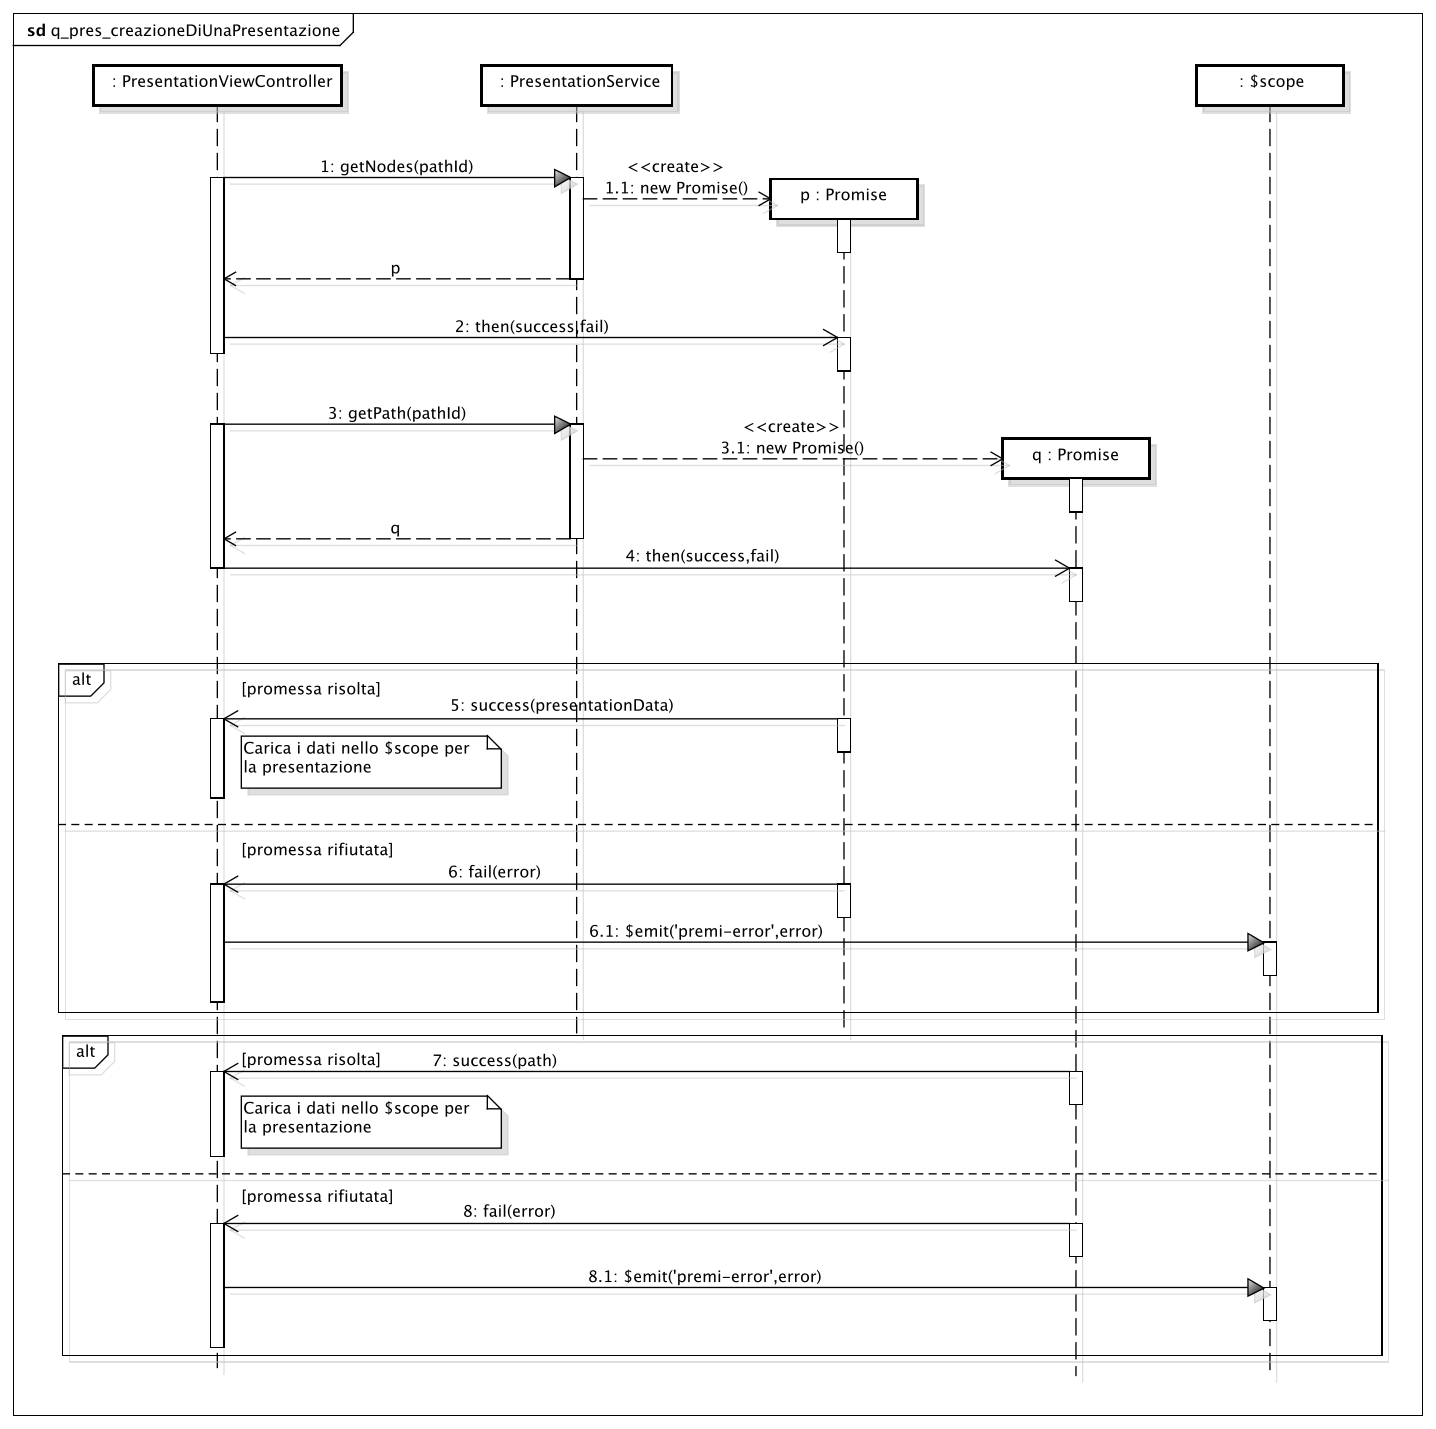
\includegraphics[scale=0.25,keepaspectratio]{diagrammi/sequenza/FrontEnd/controllers/q_pres_creazioneDiUnaPresentazione.pdf}
\caption{Diagramma di Sequenza - Creazione di una presentazione}
\end{figure}
\end{center}
\FloatBarrier
Quando l'utente vuole visualizzare una presentazione viene indirizzato verso la \texttt{PresentationView}, la quale permette di vedere il contenuto del \gloxy{frame} dei nodi come se fosse uno slideshow.\\
Per far si che la presentazione venga generata correttamente, è necessario che il costruttore del \gloxy{controller} della \gloxy{view} predisponga nello \texttt{\$scope} tutti gli oggetti necessari per la creazione della presentazione.\\
Come prima cosa il \gloxy{controller} deve recuperare l'\texttt{id} del \gloxy{percorso} da presentare, attraverso la variabile \texttt{\$routeParam} fornita da \gloxy{Angular}.\\
Una volta recuperato l'identificativo del \gloxy{percorso}, il \gloxy{controller} richiede a \texttt{PresentationService}, sia i nodi, sia l'oggetto rappresentante il \gloxy{percorso}, chiamando i metodi \texttt{getNodes} e \texttt{getPath}.\\
Entrambi i metodi ritornano un oggetto di tipo \texttt{Promise} al quale il \gloxy{controller} fornisce le funzioni da invocare quando vengono risolte o rifiutate.\\
Se una delle due promesse viene rifiutata, il \gloxy{controller} solleva l'evento \texttt{premi-error} per segnalare all'utente che non è stato possibile caricare la presentazione.\\
Se invece entrambe le promesse vengono soddisfatte, il \gloxy{controller} carica nello \texttt{\$scope} tutti i dati necessari alla directive \texttt{premiPresentation} per generare la presentazione.
